\documentclass[10pt,letterpaper]{article}
%\documentclass{sig-alternate}
\usepackage{times}
\usepackage[letterpaper, margin=1in]{geometry}
\usepackage{listings}
\usepackage[T1]{fontenc} % fonts in T1 seem to look nicer, esp for listings
\usepackage{txfonts}  % apparently needed to fixup the formatting of lstlistings
\usepackage[protrusion=true,expansion=true]{microtype} % improves text layout
\usepackage{multicol}
\usepackage{xspace}
\usepackage{color}
\usepackage{url}
\usepackage{graphicx}

% tldrs
\usepackage{wrapfig}
\usepackage{tcolorbox}
\usepackage{lipsum}
\newenvironment{tldr}[1][r]
  {\wrapfigure{#1}{0.33\textwidth}\tcolorbox}
  {\endtcolorbox\endwrapfigure}
\newenvironment{textfig}
  {{0.75\textwidth}\tcolorbox}
  {\endtcolorbox}

\lstset{
basicstyle=\ttfamily\footnotesize,       % the size of the fonts that are used for the code
numbers=left,                   % where to put the line-numbers
numberstyle=\ttfamily,      % the size of the fonts that are used for the line-numbers
%aboveskip=0pt,
%belowskip=0pt,
stepnumber=1,                   % the step between two line-numbers. If it is 1 each line will be numbered
%numbersep=10pt,                  % how far the line-numbers are from the code
breakindent=0pt,
firstnumber=1,
%backgroundcolor=\color{white},  % choose the background color. You must add \usepackage{color}
showspaces=false,               % show spaces adding particular underscores
showstringspaces=false,         % underline spaces within strings
showtabs=false,                 % show tabs within strings adding particular underscores
frame=leftline,
tabsize=2,  		% sets default tabsize to 2 spaces
captionpos=b,   		% sets the caption-position to bottom
breaklines=true,    	% sets automatic line breaking
breakatwhitespace=true,    % sets if automatic breaks should only happen at whitespace
columns=fixed,
basewidth=0.52em,
xleftmargin=6mm,
xrightmargin=0mm,
numberblanklines=false,
language=Scala,
escapeinside={(*}{*)}
}
% \lstset{
% framexleftmargin=15pt,
% basicstyle=\footnotesize
% }


\newcommand{\jmh}[1]{{\textcolor{red}{#1---jmh}}}
\newcommand{\vikram}[1]{{\textcolor{blue}{#1---vikram}}}

\newcommand{\eat}[1]{}

\author{
Joseph M. Hellerstein\\
       {\scriptsize hellerstein@berkeley.edu}
}
\title{Grounding Big Data with Metadata Services}
\date{}

\begin{document}
\maketitle

\begin{abstract}
\emph{Ground} is an open-source metadata service under development at UC Berkeley.  Ground is motivated by our experiences with users of open-source data processing packages like Spark, Hadoop and Jupyter, and the software vendors that provide tools and services in those ecosystems.  We have repeatedly heard requests in those communities for a flexible, vendor-neutral, open-source metadata service.  An overriding theme in these discussions is that the way we use data has changed philosphically and practically in the last decade.  This makes the requirements for metadata services both more urgent and quite different than they were in previous generations.

This document presents the motivation and architecture of the Ground service.  A companion document presents \emph{Common Ground}, the metamodel for Ground~\cite{commonground}.  A prototype implementation of Ground is in active use in a deployment at UC Berkeley managing metadata for a large undergraduate course.  Although the prototype is functional, we expect that Ground will require new technical developments in a number of areas; an early focus is to design a new kind of database to handle Ground's unique metadata workloads efficiently.
\end{abstract}


\section{Metadata in a New Era}
\label{sec:intro}
Our working relationship with data has changed substantially from the models established in the 20th Century.  There are many forces driving these changes, but they move us collectively in the same direction: data is no longer treated as an accounting of Truth, but rather a raw material that can be transformed and interpreted to provide value.  
%\jmh{Maybe Constructivist is a more specifically appropriate term.  Probably too esoteric though.}   
This shift points toward the need for a new foundational service that captures the \emph{metadata} describing how data is interpreted---a network of the datasets, code and people who use them over time.  We are building a prototype of this kind of service that we call Ground.  This document captures the initial motivation, design, status and plans for the Ground metadata service.

\subsection{The New Metadata Syllogism: Context is King}

Before we describe Ground, we review the forces of change in the way that many organizations work with data.  This discussion, while relatively non-technical itself, has significant technical relevance, particularly as it calls into question some of the basic tenets of traditional 20th Century data management that arose out of corporate Information Technology (IT) use cases.

First, data and computation have become affordable commodities over the past decade. Moore's Law captures the underlying hardware economics, but the progress of the last decade is best seen in a broadly increasing ecosystem of high-level services including inexpensive storage, public cloud computing, open source software, cheap and high-frequency sensing (the ``Internet of Things''), and increasingly intelligent software and user interfaces for working with data.  It takes very little capital or time to get going with data today in a big way.

Second, with a breadth of access to data comes a breadth of use cases for working with data---far more diverse and creative than the corporate IT tradition of accountancy and reference information.  Different actors (people, departments, organizations) bring a diversity of goals and assumptions to their work with data, and have incentive to use data and computation in diverse ways to further those goals.
%\footnote{Interestingly, this diversity occurs for an individual actor over time: incentives, goals and assumptions change as their tasks shift from basic record-keeping to exploratory analysis and operationalization of services.}.

Third, with a diversity of motivations comes a diversity of transformations and models for data.  In traditional IT use cases, data and databases were seen as an accounting of objective Truth; today they are increasingly viewed through a contextual or relativist lens.  Data is no longer viewed as a single Truth; it is parsed, modeled, transformed and analyzed differently for different purposes.  This leads to many different interpretations of data.  It also leads to different appreciations of data: the \emph{veracity} of data is often less important than its \emph{value}, realized through usage.

We summarize this argument as a syllogism in Figure~\ref{fig:syllogism}.  Computationally, what all this means is that the most valuable aspect of data is the context in which it is used: by whom, with what models and assumptions, and to what ends.  In information theory terms, the most important bits that we store are the ones that capture this context: \emph{the metadata}.  Unfortunately we're not doing a good job modeling or capturing these bits today---the subject of our next section.

\begin{figure*}[t]
\begin{centering}
\begin{tcolorbox}[width=0.75\linewidth]
\begin{enumerate}
\item Data and computation have become commodity resources with high value.
\item Commoditization enables diverse actors to work with data.
\item Each actor's incentives determine how they interpret and use data.
\item Interpretation and usage determine the meaning and value of data.
\end{enumerate}
Result: The meaning and value of data is not intrinsic, it is contextualized by interpretation and usage. Systems for data management need to capture this context by associating data with people, models, interpretations and usage. 
\end{tcolorbox}
\end{centering}
\caption{As data usage is commoditized, metadata becomes a central requirement.}
\label{fig:syllogism}
\end{figure*}



\subsection{Structure, Play and the Evolution of Metadata Needs}
Our discussion up to now has looked at large-scale trends and philosophy.  Next we shift to a more pragmatic look at the evolving software ecosystem for data management, to understand why metadata is so poorly served today.

``Big Data'' has been the rallying cry of much of the change in our relationship with data over the past few years.  
%Few people will admit to liking the phrase, but it accurately captures an enthusiastic ethos of More! Bigger! Faster! (or ``Variety, Volume and Velocity'' if you prefer industry analyst mnemonics.)  The Big Data ethos was driven by Internet services like search engines and social networks over the course of more than a decade, and it has led to substantial shifts in the way that data analysis software is designed and data is analyzed.
The center of the open-source Big Data ecosystem is Apache Hadoop, which recently celebrated its 10th anniversary.  There is much to admire about Hadoop, but perhaps its most important accomplishment is the vibrant open-source community that has rallied around it, building new software components for a variety of uses. The Hadoop ecosystem is evolving so quickly today that there is growing confusion about what software precisely constitutes Hadoop.  This ambiguity illustrates the most important---and difficult---changes brought about by the Big Data ecosystem, which center around agility and ``play'' in the designs for data and systems.  

The Big Data ecosystem has from its early days rejected fixed structures in favor of agility and flexibility.  This has had both positive and negative implications.  We look at the pros first:
\begin{itemize}
\item \textbf{Flexible data models and usage.} Hadoop began with a rejection of fixed structures for data.  Where previous data systems imposed some data model with more or less structure, Hadoop chose to deal with least-common-denominator raw files and ``schema-on-read'' semantics: each computation imposed its own model and structure on data in an ad-hoc fashion.  This has fueled a healthy diversity of usage in the Big Data ecosystem, which tends to celebrate analytic applications like product recommendations, news article analysis and computational genomics over bread-and-butter accounting tasks like inventory tracking.
\item \textbf{Flexible software architecture.} Over time Hadoop also rejected traditional data systems software structure as well, though this only became widely understood in recent years.  Previous data management systems were tightly-coupled software ``smokestacks'' supporting queries, storage, metadata, etc. underneath a single API and query language.  The openness of the Big Data software architecture has led to a vibrant ecosystem of open source engineering across Internet services, software vendors, academic groups and volunteers.  In today's Hadoop stack, it is possible to mix and match storage systems (e.g., HDFS, HBase, Kudu, Isilon) compute frameworks (e.g., MapReduce, Spark, Impala, Drill, Tez, Flink, Hive, Pig, etc.) and schedulers (e.g., YARN, Mesos), among other more minor swappable components. 
\end{itemize}

While there have been undeniable positive aspects of the ``play'' in open source Big Data, it has had some cons as well, increasing the challenges for interoperability and learning---across both machines and humans.
\begin{itemize}
\item \textbf{Undocumented state.}  In the absence of common data models and software, it is difficult to know much about the state and history of a given Big Data installation.  Even simple features that we used to take for granted in the past---e.g., a catalog of the data in a single repository---have become difficult.  This difficulty is far worse when trying to achieve more complex goals, like establishing data lineage or enabling components and applications to interoperate.
\item \textbf{Undocumented usage.} In the absence of common infrastructure for sharing information, current Big Data components do little to expose their own ``exhaust''---information about their inputs, outputs and usage---in reusable ways.  Hence it is currently difficult for humans or algorithms to analyze the usage of data and the behavior of systems and people using data in an organization, because the usage information---and the connections of that usage to data---are not easy to capture across the ecosystem.  In short, the Big Data software ecosystem is not learning from its own usage.
\end{itemize}

The loose structuring of the Big Data ecosystem is arguably its most important feature and its most important weakness.  It seems far more of a distinguishing factor from prior generations than technicalities like mid-query fault tolerance, compressed documents, programming models, or in-memory processing. 

Most importantly, the play in the architecture of Big Data software breaks the mold---we will not be going back to closed-source smokestack solutions with fixed data models any time soon, because the developer and user ecosystems have become used to the open source flexibility and pricing models, and the rapid rollout of new features via agile development.  With the Big Data revolution well underway, we need to design additional services to ameliorate its weaknesses: in particular we need a common, shared metadata service layer to allow this diverse ecosystem to describe itself, measure itself, and foster interoperation.

% In sum, for reasons of technological philosophy and pragmatism, we need a new generation of metadata services to ground the Big Data software arena.  Talking with developers and users of the current Big Data stack it is also very clear that we need it as soon as possible.

\section{Design Tenets and Architectural Decisions}
\label{sec:designreqs}
We believe that the relativist view of data will become dominant over time, and that the software ecosystem for data will continue to be diverse and evolving.  This leads to four key tenets for the design of Ground:

\vspace{0.5em}\noindent
\textbf{Tenet 1: Immutability and versions.}  The traditional idea of mutable storage---updating ``old'' data with ``new'' or ``fixed'' data---is incompatible with a relativist view: it erases history and discourages diverse interpretations. Instead, it is preferable to enable a multi-version approach to data update.
Ground needs to support this working style by tracking versions of data and code as they evolve over time.  This includes providing a versioning capability for systems that do not provide it instrinsically (e.g. HDFS), and integrating with a variety of versioning systems that are in use (Git, Subversion, etc.)  The metadata that Ground stores needs to be versioned as well, so that the big picture of a dataset---its raw bits as well as its metadata---are tracked consistently over time.

% The traditional objectivist notion of a database as ``the facts'' was consistent with a temporal lens of ``the present'': ``the facts as we know them today''.  In that model, if we should learn that something in the database is ``wrong'', we should ``fix'' it by replacing it with correct information.  This made especially good sense when storage was expensive.  But today storage is cheap, and our use of data is relativistic, so there is no sense in overwriting data with ``up-to-date'' or ``more correct'' information.  We should maintain as many versions of data as we find cause to interpret, and we should keep them around so we can interpret the history of the data as well. But all this only makes sense if we track the version history so we can understand how different versions got generate and used, and how version histories are intertwined across objects and use.

\vspace{0.5em}\noindent
\textbf{Tenet 2: Robust Modeling.}  The open source ecosystem is designed to foster decentralized innovation and change, so a common metadata service needs to be robust to shifting needs and designs in the services it support. To this end, we can be guided by the success of the Internet architecture, and particularly Postel's Law of Robustness:
\begin{quote}
\emph{Be conservative in what you do, be liberal in what you accept from others}~\cite{postel}.
\end{quote}
In particular, the metadata model (metamodel) and APIs for Ground needs to be very simple and very permissive, to accomodate diverse designs of core concepts including versioning, data models, and data lineage.

\vspace{0.5em}\noindent
\textbf{Tenet 3: The Centrality of Usage and Lineage.}  Since the value of data is determined by its interpretation and usage, it is critical to track the usage of data over time.  In addition, the result of many data-centric tasks is to generate new data sets; the lineage of these data sets (their input data, code, and the history of their generation) is key to understanding their value. In a services supporting diverse systems above it, usage and lineage will come in different forms and at different granularities; like other metadata, the modeling of data lineage needs to be both permissive and scalable.
% By admitting usage logs and data lineage as critical metadata, Ground takes on the responsibility to operate at enormous scale---usage logs are often the biggest data sets in any organization.
% Versions and models track the state of things: ``who'', ``what'' and ``when''.  Lineage is a separate and critical aspect of metadata, capturing causes and influences:``how'' and, with sufficient richness, ``why'' or even ``why not''~\cite{lineagesurvey}. 

\vspace{0.5em}\noindent
\textbf{Tenet 4: Neutrality.}  The previous three tenets are technical; this last one is more socio-economic.  In a decentralized ecosystem of software and data, a metadata service can serve as common ground, but only if it is broadly adopted.  Naturally there are diverse and sometimes competing incentives in any broad ecosystem, which can work against broad adoption.  The chances of reaching the critical mass desirable for a common service are substantially increased if the software is developed in an open-source and vendor-neutral environment.  
%Ground is beginning as an open-source project at Berkeley in the tradition of Postgres and Spark, with initial use cases coming from education and science.

% To enable widespread, the tenet of Conservative Modeling needs to be complemented by a socio-economic neutrality as well. In To foster a trust leading to adoption. it's most natural that the shared services be developed in an open source and vendor-neutral environment.\footnote{Arguably the best alternative is the benign dictatorship in particular ecosystem: Amazon could succeed at this in the AWS environment, Microsoft in the .Net/Azure environments.  In the Apache universe, though, it probably has to be vendor neutral open source.}

In addition to these four design tenets, there are four more technical architectural decisions that are critical.

\vspace{0.5em}\noindent
\textbf{a. Platform-As-A-Service.}  Ground provides a service that we expect to be used by a variety of applications and components on an ongoing basis over long periods of time.  As a result we have architected it as a service with a narrow API, which can be hosted either in a cloud environment or in a private cluster alongside other Big Data services like Hadoop. Following terminology from software-defined networks, Ground provides one API facing ``northbound'' to client components and applications, and another API ``southbound'' to a set of service components that enable Ground to function.  As we discuss later in this section, some of the southbound components may be well-served by existing open-source solutions, others may require further research and development.

\vspace{0.5em}\noindent
\textbf{b. Interoperability via facts on the ground.}  
% We are designing Ground to be a vendor-neutral platform with an open-source reference implementation.  The goal is to foster a healthy platform for other components to be built upon, whether they be open-source or closed, free or commercial.  
Interoperability of diverse components and integration of data representations is an ongoing challenge in computing. Ground is designed to enable interoperability by providing a robust, neutral environment. The design is not intended to explicitly achieve interoperability of specific services.  While this could be attempted via universal models and standards committees, we believe it is more likely that de facto standards will emerge and evolve naturally through pragmatic use and contributions from both users and software vendors.  We intend to seed this process by integrating components that we frequently use into Ground, including Spark, Jupyter, and git.

% With respect to metadata representation and interoperability, we believe that the era of ``value-added connectors'' between systems is over---this was an economic inefficiency that no longer makes sense in an era where many of the software providers give away their code for free.  Instead we plan to embrace the late-bound, agile approach that is native to the open source Big Data ecosystem.  Rather than assemble multiple parties to design standards, we hope to foster an ecosystem where de facto standards can emerge and evolve naturally through pragmatic use and contributions from both users and software vendors.  

\vspace{0.5em}\noindent
\textbf{c. Performance and reliability characteristics.} Most data-centric tasks consume and/or generate metadata, so a successful metadata service will have to be ``in the loop'' but not ``in the way''.  I particular it must provide low latency response, high availability, and reliable data durability.  In addition, by admitting usage logs and data lineage as critical metadata, Ground takes on the responsibility to operate at enormous scale---usage logs are often the biggest data sets in any organization.
% since have admitted usage logs and lineage as metadata, Ground will be called upon to scale up to enormous ingest volumes and large-scale analytics, because metadata connects all things -- and includes potentially massive usage logs.  As a result, we need to design for latency, availability, scalability and durability.  
These concerns have all been a part of the Big Data ecosystem since its inception, so in some cases we can lean on existing southbound software packages to achieve these goals.  There will undoubtedly be components, however, where Ground will have to take responsibility for these issues via new designs and implementations.

\vspace{0.5em}\noindent
\textbf{d. Agile Design}
Metadata services can get very complicated very quickly.  We will follow agile design methodology, building a Minimum Viable Prototype and iterateing quickly to get feedback and improve our understanding of the requirements and design space for metadata services.  To that end we will begin to use simple, pre-existing open-source solutions to serve our Southbound APIs, even if their performance and reliability characteristics are less than ideal.  

% Another aspect of agility is to serve a meaningful use case early in the lifecycle of the project.  We discuss initial hypotheses along these lines in Section~\ref{sec:initialuse}.


\section{Many Use Cases for Modern Metadata}
Metadata can seem like a simple issue.  Indeed, in early database systems, metadata was limited to a ``catalog'' or ``data dictionary'' that simply recorded the basic objects stored in a system. Before we discuss the architecture of Ground in more detail, we classify some of the use cases we are seeing for metadata in a modern context.

\begin{itemize}
\item {\bf Data inventory}: Like traditional metadata services, we need to provide facilities to store basic information about the data of interest, including how it is named, typed, structured and accessed, 
and summaries of its content.

\item {\bf Model-based interpretation}:  
%Traditionally, the word ``modeling'' has had separate meanings in the fields of databases and statistics.  The database community traditionally focused on data models and schemas (relational, hierarchical, semi-structured, etc.), as well discrete semantic models (ontologies, dictionaries); analytical software from the statistical community focus on statistical models, physical models, and the methods (learning, inference) that connect them to the consumption and production of data.
A goal of Ground is to capture models as first-class entities, and provide orthogonality between models and data.  This encompasses a breadth of database models for representation of data (e.g., relational, semistructured, linked, etc.) and mathematical models for describing and predicting the process generating the data (e.g., statistical or physical models).

\item {\bf Usage}:
 % Motivation: Many big data environments are designed to support analytic workloads, including both exploratory analytics (e.g., charting or ad hoc statistics), as well as production analytics workflows (e.g., log processing or model serving).  In these environments, it is useful to track
 In addition to capturing the basic intrinsic attributes of data, we also want to capture information about its usage: the way data is transformed and analyzed both by ad-hoc manual efforts and programmed workflows.  This usage information can be valuable to a number of goals, some of them quite traditional (e.g. audit logs for governance), others more novel (e.g. query logs for learning statistical models of user expertise or data utility).
 %It can also enable a host of interesting new functionality, including the modeling and mining of analytic activity within an organization to improve efficiency, identify expertise, and detect institutional biases.
 %Key aspects of this use case include \emph{activity tracking}, \emph{data lineage} and \emph{.

\item {\bf Reproducibility}:
% It is well appreciated that data sets are growing and become more widely used.  Analytic methods for these data sets are becoming increasingly intricate, both in their computational goals and in the variety of tools and libraries they use to go from ``raw data'' to ``results''. Reproducibility of analytic pipelines is a critical aspect of managing this complexity.
We want to enable reproducibility of complex workflows that generate data products. As a feature, Reproducibility has many virtues.  Primarily it fosters confidence in the veracity of results from complex data processing.  Reproducibility also enables reexecution of workflows after emending the data, models or software used in a data-centric process.  This serves over time to enable ``data debugging'', ``what-if'' analysis and evolution of data interpretations.

\item {\bf Interoperability}: An ongoing source of frustration in data processing is the inability of tools and organizations to interoperate.
%Traditionally, interoperability was achieved via standards; this was a time-consuming and political process.  In principal, widely-adopted and open source solutions like Hadoop, Spark and Jupyter should allow interopability to occur via open source and network effects.  As certain APIs and formats become mature and widely used, they serve as centers of gravity, and many systems begin to adopt them.  We have seen some of this activity around storage formats like Avro, ORC and Parquet.
A goal of Ground is to provide an environment where data interoperability can occur de facto in an open  fashion, via open source implementations and network effects.  This is similar to the emergence of formats like Avro, ORC and Parquet for data storage, but at the higher semantic level of data modeling to capture the interpretation and use of data across users and applications.

\item {\bf Collective governance}: A common role for metadata is to help \emph{govern} the use of the data it describes.  That includes modeling principals (e.g., users, groups, roles) and rights (e.g., read, update, create, execute, grant), capturing policies to be enforced (e.g., based on attributes of principals, data contents, location, time-of-day, etc.), and auditing user behavior for post-hoc analysis.
%Traditional IT environments place the creation and management of this governance metadata in the hands of ``superusers'' of one form or another, typically IT staff.  In many analytic environments today, a different approach is preferred, which distributes this authority much more broadly and flexibly to end-users who understand the data that is arriving and the experiments being performed.  Between these poles, ``curation''is needed to help data evolve smoothly from raw materials to widely used reference.
A goal of Ground is to provide a framework for a diversity of data governance philosophies, from the top-down control seen in traditional IT environments, to emergent ``collective'' governance models that foster end-user exploratory work and Wikipedia-style community curation.
 % In those agile environments, the principals best suited to assess data are not the IT superusers, but rather the end-users who understand the data and its use deeply.  For those environments, Wikipedia is a better model than traditional IT governance structures.  In many cases, a mix of governance models emerges, to ``lock down'' data sets that are known and sensitive, while simultaneously fostering ``sandboxes'' and ``landing zones'' for more agile useage.  As data migrates from ``landing zone'' to ``lock-down'', intermediate models can be advantageous to ``curate'' data
\end{itemize}


\section{Ground Architecture}
% In Section~\ref{sec:designreqs} we highlighted the high-level considerations of our design for Ground.  Here we get more granular.  We begin by focusing in on some basic design decisions, and then shift to a more detailed breakdown of the key services that make up Ground.
% \subsection{Ground Internal Architecture}
%%%%%%%%%%%%%%%%%%%%
Ground is composed of a foundational metamodel and the sub-services that back it up.  The metamodel and its Northbound API are critical: they define the Ground surface and semantics, reflecting the new data practices we wish to capture and enhance.  Metamodel definition and support represents the first code we are writing for Ground, and we expect to continue to maintain and evolve it over time.  Behind the metamodel is the Southbound API to five basic services described below.  

We are currently in the midst of an agile development cycle, building and releasing a Minimum Viable Prototype (MVP) of Ground that we call \emph{Ground Zero}. Where appropriate we describe our goals and status for the MVP separately from the longer-term discussion.  A sketch of the Ground Zero architecture is provided in Figure~\ref{fig:layers}.

\begin{figure}
\centering
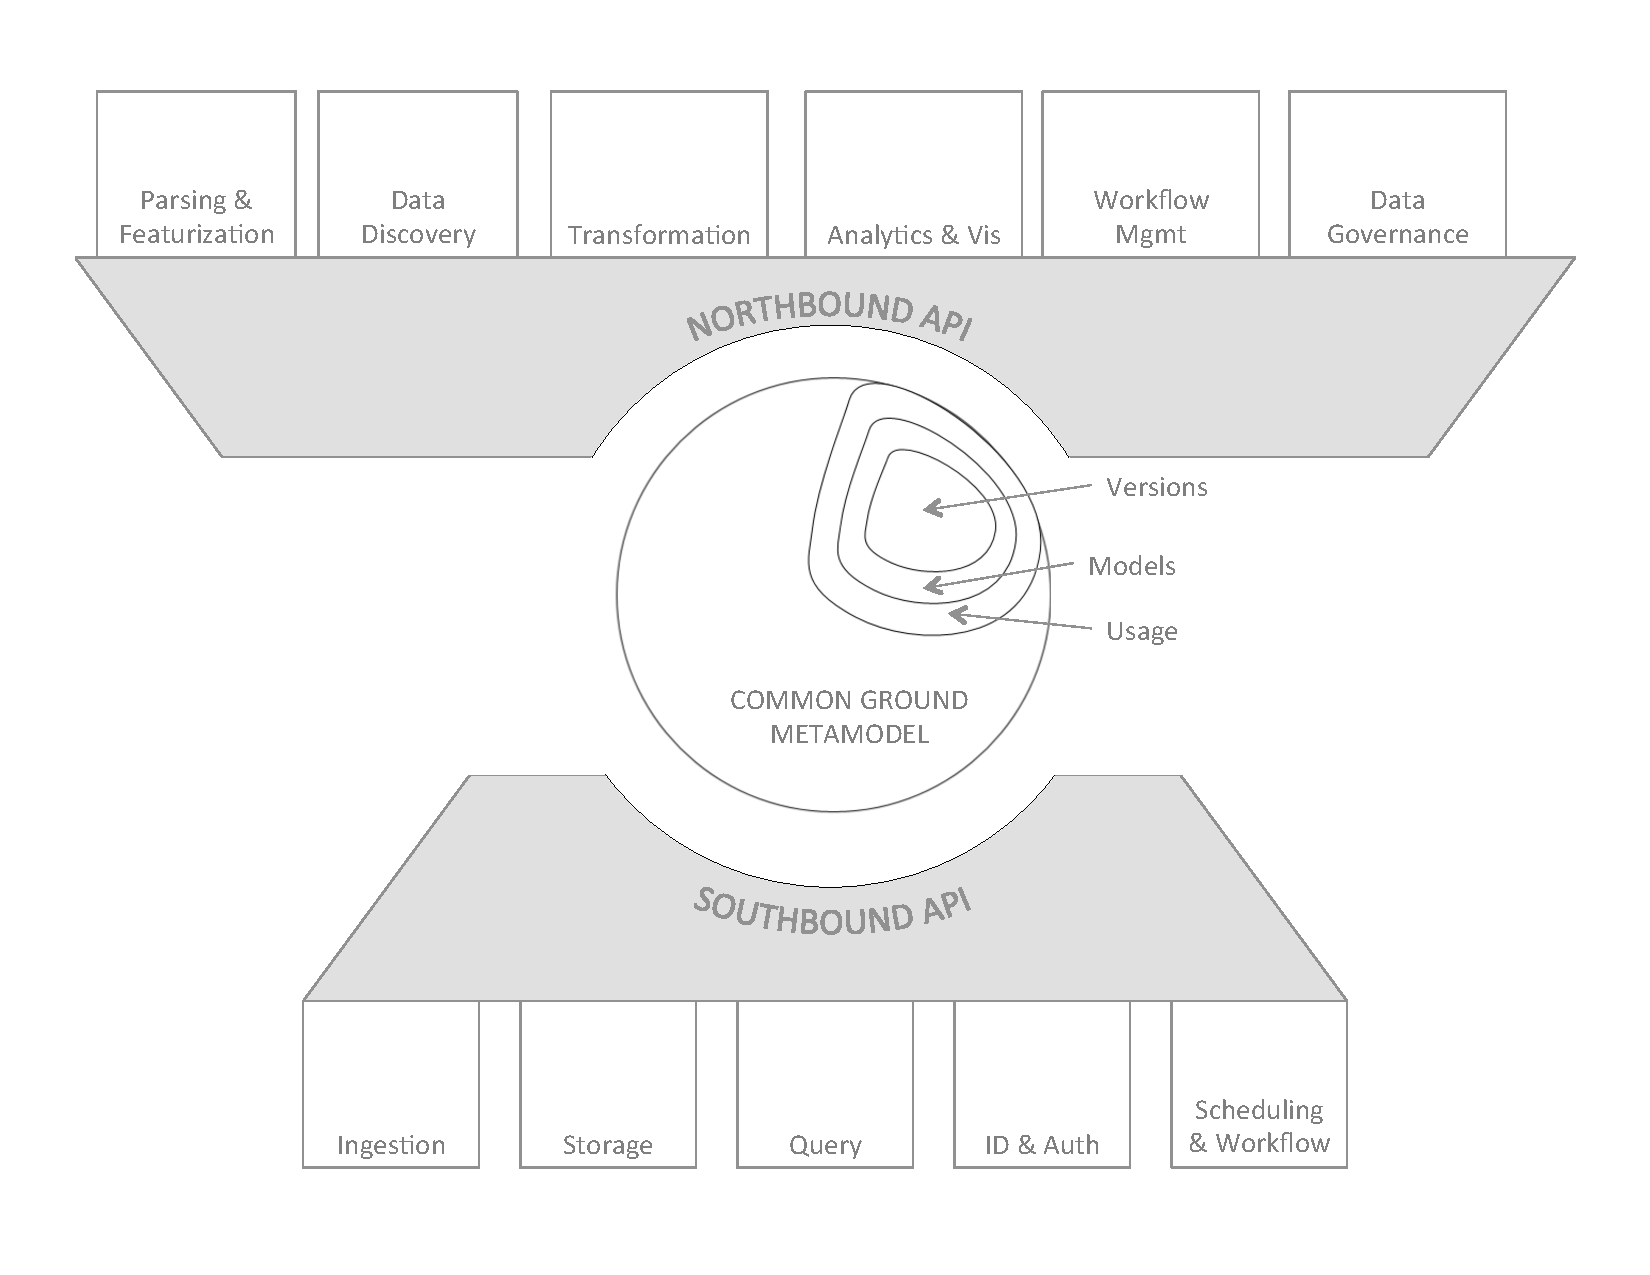
\includegraphics[width=0.75\linewidth]{ground0fig.pdf}
\caption{A sketch of the Ground architecture.}
\label{fig:layers}
\end{figure}

\subsection{The Common Ground Metamodel, In Brief}


We begin with an overview of our metamodel, \emph{Common Ground}, which is described in detail in a companion document~\cite{commonground}; we provide an overview here.  Common Ground provides a three-layer metamodel, with three intertwined graphs capturing versioning at the \emph{core} of the model, metadata modeling at the intermediate \emph{mantle} level, and usage information at the outer \emph{crust} layer.  The core versioning model supports arbitrary DAGs of versions that can be managed in Ground, or be shadowed from external versioning systems like Git. All metadata in Ground is intrinsically versioned. The mantle modeling layer offers an inclusive graph representation that can capture metadata that is represented in both structured and unstructured forms side-by-side, subsuming standard models like Relational, JSON documents, key-value stores and XML.  Usage logs, principals and lineage DAGs in the crust are the third key aspect of the metamodel, enabling the tracking of lineage across both nodes and edges in the underlying models.  The interested reader is referred to the Common Ground design document~\cite{commonground} for more detail.

A prototype implementation of Common Ground has been implemented in Scala and is in active use in a deployment at UC Berkeley managing metadata for a large undergraduate course on Database Systems with 500 students and 10 staff. It is tracking metadata about user identity across three authorization systems at Berkeley, workflows and scripts in Python, SQL, PySpark and Jupyter Notebooks, and code versioned externally at GitHub.  This prototype of the metamodel forms the initial basis of the Ground Zero MVP, and has driven the prototypes of some of the services described next.

\subsection{Key Services}
Ground's functionality is backed by five key sub-services.  It was our goal for the initial Ground Zero prototype to use existing open source solutions where possible.  We expect that some of these solutions will fail, and that innovative research will be required to develop viable technology for these services at scale.

\begin{enumerate}
\item \textbf{Versioned Metadata Storage}.  Ground must work with storage in two senses: it must store versioned metadata reliably, and manage references to externally stored data as well.  Ground must be able to store metadata with the full richness of the Common Ground metamodel, including flexible version management, data modeling and lineage storage.  Ground also needs to reference external data, which can come in arbitrary form, with a wide variety of APIs.  Note that Ground is not the primary interface for accessing the data that is referenced by metadata; Ground is expected to \emph{describe} external data and track it, not serve it.  Hence Ground's most basic requirement for external data is to know how to store a unique ID for each item it tracks, and return that ID to applications that request it.  In an ideal setting, each external data item is versioned, hence each version has a unique ID.  However if the external item is mutable and not versioned, Ground generates \emph{Schr\"{o}dinger versions} lazily: each time we observe an object we assume it changes, and assign it a new version (and version ID).  This is discussed in more detail in the Common Ground design~\cite{commonground}.

\textbf{MVP:} We are currently mapping our metadata model onto a traditional PostgreSQL relational database for storage.  Graphs can be represented as relations, so we manage versions, lineage and data modeling graphs at application level above the relational model.  PostgreSQL is a fairly mature system but is not designed to meet our requirements for latency, scalability and availability. In fact we do not expect any relational solution to work well for our needs over time, as relational databases are not designed for any of the three key individual aspects of the metamodel: versioned data, polyglot data models, or rich lineage.  Unfortunately, we do not expect that solutions in the NoSQL or graph database world will fare well either, though this requires research to validate. Therefore a critical thrust of the Ground research agenda is to understand the weaknesses of existing database systems when faced with these requirements, and design a new database system that is well-suited to emerging metadata workloads. \jmh{Need to call out research hypotheses more clearly.}


\item \textbf{Search, Query, Analyze}.  As noted above, Ground is intended to be permissive in the kind of metadata it stores.  First, it needs to support a least-common denominator of unstructured tags, and provide efficient search over those tags.  To this end it needs an indexing and search component.  Second, Ground also needs to support efficient interactive behavior for applications that are inserting, updating and fetching metadata---and capture any changes in a versioned manner.  This should be provided by the metadata storage service with low latency and high throughput.  Third, we expect that metadata will produce a rich target for analytical workloads: algorithms that study what data exists over time, as well as who, how and why data gets used and gets changed.  Finally, it seems natural that some workloads will need to combine these three classes of queries, perhaps via a federated query layer above them. 

\textbf{MVP:} Initially we are not supporting search or analytic APIs; these will be added as the system evolves.  For interactive query, we can only do as well as our prototype relational metadata store.  For search, we expect that existing solutions like Solr will be sufficient for the foreseeable future; we do not expect metadata tagging and querying to exceed volumes that Solr sees in free-text indexing. For analytics, we intend to leverage Spark and GraphX as we have significant expertise in house.  However, the nature of the analytics to be done here represents a major research opportunity: what might be the value of metadata in a Big Data context, and how could that value be extracted by analytics?  Could a \emph{self-aware} Big Data ecosystem improve itself, or provide valuable insight about its usage to applications and users?  \jmh{Again, call out research.}  Finally, the requirements for a federated query layer and its design are a topic for investigation after we acquire a corpus of metadata and workloads.

\item \textbf{Ingestion: Insertion, Queues and Crawlers}.  Metadata may arrive to be stored in Ground interactively or in batches, and it may come actively (via a ``push'' insertion interface), or passively (via a ``pull'' crawling interface).  Interactive insertion of metadata needs to be supported efficiently by the metadata storage component; batch insertion should make use of queueing services to handle bulk delivery and bursty arrivals.  Passive insertion needs to be handled via a data crawler that can register metadata from external services with Ground, and see if Ground can enrich that metadata via additional software services for file parsing and feature extraction.

\textbf{MVP:}  Currently we are handling ingest solely via simple push insertion APIs that call into our metadata store via SQL.  However we envision integrating open-source solutions like Kafka for queuing, and Gobblin for crawling and data ingest from remote sources.  We are also eager to explore APIs to plug in third-party solutions for  extracting metadata from crawled data; two examples we are OpenCalais (a free automated service for entity extraction) and Trifacta (a commercial, semi-automatic solution for data transformation).  We also recognize that there are boundless R\&D opportunities here, some of which could be part of Ground, many of which should exist as standalone solutions above Ground.  \jmh{another research opening, though more about opportunities above ground.}  We look forward to integration with other research and non-research colleagues here.

\item \textbf{Identity and Authorization Integration}.  Identity management and authorization are a required aspect of the Ground service, but almost certainly one that we want to delegate if we can.  The primary reason not to ``bake in'' authorization is administrative: most organizations already have an authorization service and do not want their metadata service to impose a new one.  More importantly, authorization is a semantic notion with wide flexibility: the authorization policies of a federal defense agency are likely to be wildly different in nature from those of a marketing department doing targeted advertising, or an international consortium of scientists interested in reproducibility.  The flexible design of Ground's metamodel should make it possible for a wide variety of use cases to capture authorization metadata (ownership, auditing, content labeling etc.) and design policy over that metadata.  An open design question is whether Ground needs to \emph{enforce} policy, or merely store it.  Note that there is a subtle set of multidimensional connections between metadata versions and policy versions, particularly when the aurthorization policies of a past time are considered unsafe later---a case where good people may disagree about the virtues of immutability.

\textbf{MVP:}  The current MVP has no support for identity management and authorization.  However our initial use case has us tracking UC Berkeley student IDs, Github identities, UNIX uids from instructional computing, and associations between the three; visibility of things like grading scripts and their outputs will depend on policies regarding these identities.  In the short term we expect to integrate with Google oAuth services as exposed at UC Berkeley next, and to explore the way that policy is specified and possibly enforced in our prototpype environment.  Our longterm roadmap here remains open; we expect a need to collaborate closely with partners in application domains to get further requirements.  \jmh{Possible tie to Raluca's work here, at minimum as an example of a non-standard approach to these issues.}

\item \textbf{Scheduling, Workflow, Reproducibility}. In this domain, it is important to separate specification from execution.  We are committed to ensure that Ground is flexible and rich enough to capture the specification of workflows at many granularities of detail: from black-box executables to workflow graphs to source code.  However, we do not expect Ground to be a universal provider of workflow execution or scheduling; instead we hope to integrate with a variety of schedulers and execution frameworks including on-premises and cloud-hosted approaches.

\textbf{MVP:} We plan to begin by utilizing the scheduling and execution services provided by the Gobblin project, which supports a variety of schedulers including Quartz, Azkaban and Oozie, and execution frameworks including Yarn and Helix.  We plan to look into support for VMs and containers as well.  \jmh{Certainly could paint a research picture here, closer to the Bloom-meets-Kubernetes agenda: how will data-centric workflows be programmed in the future, especially as we look at containers, elastic services, etc?}  maybe also a connection to the Shenker/Jackson work on Declarative Datacenters?
\end{enumerate}
%%%%%%%%%%%%%%%%%%%%

\section{Getting to MVP}
\label{sec:initialuse}
%  The identification of this use case is being driven both by our experiences with users on campus in education and research, and by our experience in industry talking to industry users and commercial software vendors in the Big Data space.  

Let's be useful out of the box and foster adoption.
HCat replace/augment, Github integration for data science.
\begin{itemize}
\item flexible schema/attributes - cover JSON, Avro, Parquet not just relational.
\item versioned metadata with attribution
\item provide a solution for versioned code+data
\item execution auditing from Spark/Jupyter
\end{itemize}

\section{Planned Use Cases}
\subsection{Course Management}
Multiple auth systems, code + data, operational and non-idempotent workflows.

\subsection{Scientific Workflow and Reproducibility}
Issues of scientific validity.  Trust aside, recalibration story from Saul Perlmutter.

\subsection{Customer Behavior Analysis}
Compound Cisco and RBS use cases .... IT vs. LOB interpretations and desire for prediction.  Understanding across the organization and departmental priorities.

\bibliographystyle{abbrv}
\bibliography{groundarch}

\end{document}


\section{Fact: Diversity}
As has been well documented, data is being generated at record rates from a record diversity of sources.  At the same time, storage capacity per dollar has been growing tremendously. Net result: it's cost-effective to capture and store a wide variety of data in great volume, and ``figure it out'' post-hoc, on -demand.  Three V's blah blah.

\jmh{All 3 V's appear in the Big Data software space! Forced analogy?}

These forces have led to an unprecedented flowering of activity over the last decade in software development and research on data processing and analysis in academia and a variety of industries.  A full decade has passed since the Hadoop project officially joined the Apache Foundation.  Over that decade, the software stack for data analysis at scale has evolved and diversified rapidly.  Today there are 32 different projects tagged ``big-data'' in the Apache open source foundation~\cite{apache}.  And of course there are many more vibrant and widely-used software packages outside the Apache foundation that are used for working with data, both free and commercial, open- and closed-source, big-data and small-data.

One of the signal architectural characteristics of today's software ecosystem for data is that it is \emph{diverse and decoupled}.  Even within the Hadoop sphere, basic building blocks are decoupled and can be swapped or in some cases even coexist in the same installation.  This includes query engines (Hadoop MapReduce, Spark, Impala, Drill, Tez, Flink), storage systems (HDFS, HBase, Kudu) and cluster schedulers (YARN, Mesos). This decoupling is a major architectural departure from earlier generations of technology like relational and semistructured database systems, which provided monolithic systems that provided a full range of functionality in a single system with a single set of architectural assumptions (data model, query language, storage guarantees).  The decoupling of data system architectures has allowed the open-source ecosystem to thrive, working on independent pieces and thus moving relatively quickly through successive generations of component designs. 

This decoupling has also become a key criterion for organizations that use these technologies.  Customers have thrown off the traditional shackles of ``vendor lockin'' in their data stacks for open-source replacements, and have come to demand an ability to swap out componentry and support providers in a relatively fine-grained fashion.

This philosophy of decoupling has been carried into the data representations as well.  In most modern data management environments, data storage (the arrangement of bits in memory or on disk) is often explicitly separated from data modeling (the description of how to interpret those bits). Data can be stored with no models, to simplify data capture and support ``structure-on-read'' interpretation.  Data can also be viewed through the lenses of multiple alternative models, to support a diversity of interpretations for different use cases, often executed using different software frameworks.

Net result: today's data ecosystem accommodates a wide range of systems---including data models, language APIs and storage guarantees.  This has become the accepted status quo in the user community.  It's here to stay.



% \subsection{The Need: Grounding Big Data in Metadata}
This year marks the 10th anniversary of Apache Hadoop, and is the year that analyst group Forrester predicted that 100\% of large enterprises would eventually adopt Hadoop in some form.  For a variety of technical, economic and cultural reasons, Hadoop and related Big Data frameworks have been a radical success for open source software, thriving in a wide range of organizations from research labs to government agencies and traditional business.    

However, open-source Big Data infrastructure was originally designed to provide an interface to simple parallel computations over data files---primarily indexing and ranking web documents.  The primary focus of the initial Big Data frameworks was to support computation over unstructured files, not to manage data per se.  

This is changing quickly.  Today, Big Data infrastructures---and the data they store---are being deployed for a wide variety of purposes.  Some users  are still employing these systems for one-off applications and ``science experiments''.  But as usage broadens, organizations are deploying open-source Big Data technology to support ongoing work involving many people and projects, 
bringing a variety of motivations and goals to the same infrastructure and data.  \jmh{Cite some ambitious installations...}

The net result is that Big Data is no longer just disposable ``fuel'' for computation~\cite{dataisthenewoil}; it is a resource with its own intrinsic value that needs to be managed over time and across an organization.  A key implication of this maturation is a growing need for \emph{metadata management}: the ability to know 
\emph{what} data you have, %(cataloging, annotation), 
\emph{why} you have it, % (provenance), 
\emph{how} it gets used % (monitoring, modeling), 
and \emph{who} knows about it. % (audits and permissions). 
This information needs to be tracked across time, and evolve organically with data and its usage.

Metadata has traditionally been a feature of data infrastructure.  However the modern Big Data ecosystem brings a variety of novel challenges that center on \emph{diversity}:
\begin{itemize}  
\item \textbf{Software diversity:} 
%Metadata was traditionally managed within the same system that supported data storage and computation---e.g. a relational database.  Big Data infrastructures explicitly decouple storage from computation. 
In the modern Big Data stack it is possible to mix and match storage systems (HDFS, HBase, Kudu, Isilon) compute frameworks (MapReduce, Spark, Impala, Drill, Tez, Flink, Hive, Pig, etc.) and schedulers (YARN, Mesos).  Above and adjacent to these frameworks are a growing variety of value-added applications ranging from broad-purpose data transformation, visualization and analysis packages to application-specific tools for tasks like customer segmentation, product recommendation and so on.
As a result, metadata management needs to be an independent service that can run alongside all of these components and handle their metadata in natural ways.
\item \textbf{Modeling diversity}: In today's data rich environment, most data does not provide a ``golden master'' accounting of accepted truth.  Instead, data is often used as evidence for inference and prediction.  In many cases, the same raw data is transformed into multiple distinct formats to feed multiple models associated with distinct applications.  This diversity of modeling affects both the structure and interpretation of data.
\item \textbf{Computational diversity}: richness of computation.  
\item \textbf{Organizational diversity}: Offload of IT.   Who decides on the policy and value around data.  Governance, Curation, Reproducibility.
\end{itemize}






Agile engineering ... start with an MVP called ``Ground Zero'' that leverages existing open source components, use it to build to a reference architecture.  Then identify shortcomings for our needs, and innovate where we most need to.  At this early stage we have strong suspicions that major challenges will arise at our storage layer, due to our desire to support immutable, archived metadata that carries the version history and data lineage of every object of data or metadata that we track.

Note that metadata services have broad and stringent requirements.  They can end up on the critical path of systems that need to be lightweight (think auth/governance use cases), and also can be called upon to provide high-volume ingest and analytics behavior (think usage logs and recommendation services). So metadata services may have to match the most stringent latency and availability requirements of the interactive applications they serve, while also dealing with the data volumes seen in Big Data analytics.  


In modern data-driven organizations, data is no longer treated as an accounting of Truth, but rather a raw material that is transformed and interpreted for multiple purposes.  In a very practical sense, data is no longer meaningful without understanding the context of its usage.  This relativist view points toward the need for a new foundational service that captures the metadata describing how data is interpreted -- a network of the datasets, models, code and usage of data by people and organizations over time.  We are designing a new metadata service layer called Ground, which is targeted at tracking this information in the Big Data open source ecosystem.  In keeping with the relativist view of data, Ground’s metadata storage is founded on an immutable versioning scheme that can track the many ways that the referenced data gets transformed and used over time.  To track context, Ground can keep metadata on both data sets and software code bases, as well as the lineage of data products that are the result of running code over data, as well as data usage.  To foster interoperability, Ground is based on Internet design tenets favoring simplicity of modeling to accommodate a broad range of   
